\subsection{Set up}

Density functional theory (DFT) was used to do the calculations in this report. The functional used was Perdew-Burke-Ernzerhof (PDE) functional which is a type of Generalized Gradient Approximation (GGA) functional. The program used was the Vienna Ab initio Simulation Package (VASP) \cite{vasp1,vasp2,vasp3,vasp4}.


\subsection{Execution}

\begin{itemize}

\item Found structure for $\beta- \text{Ga}_2\text{O}_3$

\item Checked convergence for energy cut-off and k-point density for primitive unit cell

\item Relaxed the unit cell (both ions and cell)

\item Plotted local and total DOS for primitive unit cell

\item Found high symmetry k-points in structure

\item Plotted band structure for primitive unit cell

\item Made supercell (1x 3y 2z) of 120 atoms

\item Relaxed structure (only ions)

\item Changed convergence criteria, to lessen the CPU time

\item Relaxed supercell (both ions and cell)

\item Calculated energy for relaxed supercell

\item Made three different structures for three different oxygen vacancies

\item Relaxed all three structures

\item Calculated energy for the relaxed structures

\item Relaxed the O$_2$ in vacuum

\item Calculated energy of relaxed oxygen molecule

\item Found formation energy 

\item Investigated electron density isosurfaces visually

\item Plotted local DOS of neighboring gallium atoms

\item Compared with local DOS in normal supercell


\end{itemize}

\subsection{Convergence}

This subsection present the result from the convergence tests. The figures have normal convergence criteria plotted with the results, to help evaluate them. 

\subsubsection{Energy cut-off}

\begin{equation}\label{eq:relative_energy}
|\Delta E_{rel}^i| =\left| \left( E_a^{i+1}-E_a^i\right)-\left( E_b^{i+1}-E_b^i\right)\right|
\end{equation}

We started with convergence with respect to energy cut-off. Figure \ref{fig:totencutoff} shows the plot of the change in relative energy, $\Delta E_{rel}$ (see Equation \ref{eq:relative_energy}), between the total energy of the primitive unit cell, $E_a$, and the total energy of the unit cell with one less oxygen, $E_b$, against the cut-off energy. The plot shows that a cut-off energy of 600 eV would give a good convergence well below 1 meV for the energy.

\begin{figure}[H]
\includegraphics[width=\linewidth]{../fig/deltatotencurverel.pdf}\caption{This is a plot of the difference between change in energy for $\beta \text{-Ga}_2\text{O}_3$ with and without a oxygen vacancy. We can see from the plot that a cut-off energy of 600 eV is sufficient.}\label{fig:totencutoff}
\end{figure}

We also looked at the force and the pressure with respect to the cut-off energy. Figure \ref{fig:forcepresscutoff} shows the result. A cut-off energy of 600 eV gives a good convergence for force and pressure also. 

\begin{figure}[H]
\includegraphics[width=\linewidth]{../fig/deltaforcepressrel.pdf}\caption{This is a plot of the difference between change in both force and pressure for $\beta \text{-Ga}_2\text{O}_3$ with and without an oxygen vacancy. We can see from the plot that with respect to pressure and force 600 eV is more than sufficient. The change in force increases, but it is still small.}\label{fig:forcepresscutoff}
\end{figure}

After increasing the primitive unit cell to a super cell, the CPU time of the relaxation increased a lot. To make the calculations more workable, the convergence criteria was made a little less strict and the new cut-off energy was sat to 500 eV. When we look at Figure \ref{fig:totencutoff} and \ref{fig:forcepresscutoff} we see that a cut-off energy at 500 eV gives a good convergence as well, it is still around 3 meV for the energy and around 1 kbar for the pressure and 0.01 eV/Å for the force.

\subsubsection{k-point density}

Thereafter, we evaluated the necessary k-point density. Figure \ref{fig:totenkpoints} shows the result for the relative change in energy and Figure \ref{fig:forcepresskpoints} shows the same for force and pressure. 

\begin{figure}[H]
\includegraphics[width=\linewidth]{../fig/deltatotencurverel_kpoints.pdf}\caption{This is a plot of the difference between change in energy for $\text{Ga}_2\text{O}_3$ with and without a oxygen vacancy. We can see from the plot that a k-point density of 5 $\text{Å}^{-1}$ is sufficient.}\label{fig:totenkpoints}
\end{figure}

\begin{figure}[H]
\includegraphics[width=\linewidth]{../fig/deltaforcepressrel_kpoints.pdf}\caption{This is a plot of the difference between change in both force and pressure for $\text{Ga}_2\text{O}_3$ with and without a oxygen vacancy. All the k-point densities gives good convergence.}\label{fig:forcepresskpoints}
\end{figure}

Initially the k-point density was put to 5 Å$^{-1}$, for the accuracy to be at 1 meV for the energy. After the change in strictness, only 3 Å$^{-1}$ were necessary to accomplish the criteria of 3 meV for the accuracy of the energy, 1 kbar in pressure and 0.01 eV/Å in force. 

%\subsubsection{Oxygen molecule}
%
%We also had to check the convergence of the oxygen molecule in vacuum, to calculate the formation energy. Figure \ref{fig:totencutoff_O2} and \ref{fig:forcepresscutoff_O2} shows the convergence result for this with respect to energy cut-off. To get the same accuracy as for the gallium oxide super cell a cut-off energy of \ref{} eV is necessary.
%
%
%\begin{figure}[H]
%\includegraphics[width=\linewidth]{../fig/oxygen/deltatotencurverel.pdf}\caption{This is a plot of the change in the relative energy for the oxygen molecule in vacuum with respect to cut-off energy. The relative energy is the difference between the oxygen molecule with the normal bond length and a longer bond length.}\label{fig:totencutoff_O2}
%\end{figure}
%
%\begin{figure}[H]
%\includegraphics[width=\linewidth]{../fig/oxygen/deltaforcepressrel.pdf}\caption{This is a plot of the change in the relative force and pressure for the oxygen molecule in vacuum with respect to cu-off energy. The relative force and pressure is the difference between the oxygen molecule with the normal bond length and a longer bond length.}\label{fig:forcepresscutoff_O2}
%\end{figure}
%
%
%The convergence test with respect to the k-point density of the oxygen molecule is in Figure \ref{fig:totenkpoint_O2} and \ref{fig:forcepresskpoint_O2}. To get the same accuracy as for the gallium oxide a k-point density of \ref{} Å$^{-1}$ is necessary.
%
%
%\begin{figure}[H]
%\includegraphics[width=\linewidth]{../fig/oxygen/deltatotencurverel_kpoints.pdf}\caption{This is a plot of the change in the relative energy for the oxygen molecule in vacuum with respect to k-point density. The relative energy is the difference between the oxygen molecule with the normal bond length and a longer bond length.}\label{fig:totenkpoint_O2}
%\end{figure}
%
%\begin{figure}[H]
%\includegraphics[width=\linewidth]{../fig/oxygen/deltaforcepressrel_kpoints.pdf}\caption{This is a plot of the change in the relative energy for the oxygen molecule in vacuum. The relative energy is the difference between the oxygen molecule with the normal bond length and a longer bond length.}\label{fig:forcepresskpoint_O2}
%\end{figure}